% ============================================================
%  GamefyDB — PFE Report  |  Chapter 3
%  Sprint 1: Data Ingestion and Cleaning
%  Paste this block into the main document, replacing \end{document},
%  then add \end{document} at the very end.
% ============================================================

% Placeholder macro (only needed if this file is compiled standalone;
% the macro is already defined in rapport_chapters1_2.tex):
\providecommand{\todoFigure}[2][0.7\textwidth]{%
  \fcolorbox{red!60!black}{red!5}{%
    \parbox{#1}{\centering\vspace{0.6cm}%
      \textcolor{red!60!black}{\textbf{[TODO --- insert figure]}}\\[4pt]
      \textit{#2}\vspace{0.6cm}}}%
}

% ============================================================
%  CHAPTER 3 — SPRINT 1: DATA INGESTION AND CLEANING
% ============================================================
\chapter{Sprint 1: Data Ingestion and Cleaning}

% ----------------------------------------------------------
\section{Introduction}

With the preparation phase behind us, the project enters its first
implementation sprint. The work undertaken here corresponds to the two
opening stages of the GamefyDB pipeline, ingestion and cleaning, and
realises user stories US-01 through US-04 of the backlog. The deliverable
expected at the close of the sprint is a pipeline capable of opening the
four source \texttt{.xls} files without a single encoding error, removing
every layout artefact left behind by the export software, and emitting a
collection of fully typed DataFrames that the dimensional-modelling sprint
can consume directly.

% ----------------------------------------------------------
\section{Sprint 1 Goals}

Before any line of code is written, it is worth restating the goals that
the sprint commits to. They were agreed with the Product Owner during the
sprint planning meeting and shaped every technical decision that follows.

\begin{itemize}
  \item \textbf{Tolerant ingestion.} The pipeline must read the four source
        files regardless of the encoding quirks they carry, in particular
        the \texttt{charmap} error raised by \texttt{pandas.read\_excel}
        when it encounters the members file.
  \item \textbf{Artefact-free data.} Page-break sequences, repeated header
        rows, blank separators, and the footer row of the members file
        must disappear before any further treatment. The downstream sprints
        should never have to deal with these.
  \item \textbf{Native types.} Every column of every DataFrame produced by
        Sprint~1 must carry the right native Python or pandas type:
        \texttt{datetime64} for timestamps, \texttt{float64} for monetary
        amounts, \texttt{int64} for durations and identifiers, and
        \texttt{object} for textual labels.
  \item \textbf{Unified terminal naming.} The terminal name extracted from
        the parenthesised comments of the cash and stock files must match
        bit-for-bit the names used directly in the sessions file, so that
        a single conformed dimension can be built later.
  \item \textbf{Reproducibility.} Given the same inputs, the pipeline must
        return the same DataFrames on any machine, with no manual cleanup.
\end{itemize}

% ----------------------------------------------------------
\section{Sprint 1 Backlog}

The sprint backlog was extracted from the product backlog defined in Sprint~0 and
covers the four user stories related to raw data access and type normalisation.
Table~\ref{tab:sprint1_backlog} presents the tasks that were committed to this sprint.

\begin{longtable}{>{\bfseries}p{1.3cm} p{4.2cm} p{7cm}}
  \caption{Sprint 1 Backlog.\label{tab:sprint1_backlog}} \\
  \toprule
  \textbf{ID} & \textbf{User Story} & \textbf{Tasks} \\
  \midrule
  \endfirsthead
  \toprule
  \textbf{ID} & \textbf{User Story} & \textbf{Tasks} \\
  \midrule
  \endhead
  \bottomrule
  \endfoot

  US-01 & As an analyst, I want the pipeline to read all four source files
          without encoding errors.
        & Implement \texttt{ingest\_all()} using \texttt{xlrd}; define
          \texttt{COLUMN\_MAPS} from empirically verified column positions. \\[4pt]

  US-02 & As an analyst, I want all page-break artefacts removed automatically.
        & Implement \texttt{\_strip\_artifacts()} to remove blank rows, page
          markers, and repeated header rows. \\[4pt]

  US-03 & As an analyst, I want TND amounts, datetimes, and durations to be
          correctly parsed into native Python types.
        & Implement \texttt{parse\_amount()}, \texttt{parse\_datetime()}, and
          \texttt{parse\_duration()} in \texttt{cleaner.py}. \\[4pt]

  US-04 & As an analyst, I want terminal names extracted from comment fields so
          that sessions, cash, and stock share a common terminal dimension.
        & Implement \texttt{extract\_terminal()} using a regular expression;
          handle nested parentheses such as \texttt{(PS5\,(1))}. \\
\end{longtable}

% ----------------------------------------------------------
\section{ETL pattern adopted for Sprint 1}

A short word on the integration pattern adopted before diving into the
implementation. GamefyDB follows the classical \textit{Extract –
Transform – Load} chain, but Sprint~1 is only concerned with the first
two boxes, illustrated in Figure~\ref{fig:sprint1_flow}. The
\textbf{Extract} step is realised by \texttt{gamefydb/ingestor.py}, which
opens the workbook through \texttt{xlrd} and rebuilds a flat
\texttt{DataFrame} from \texttt{ws.row\_values()}. The \textbf{Transform}
step is the responsibility of \texttt{gamefydb/cleaner.py}, which
normalises types and extracts the terminal name from the comment column.
The \textbf{Load} step is deliberately postponed to Sprint~2, where the
typed DataFrames produced here are assembled into the star schema and
written out as CSV files.

\begin{figure}[H]
  \centering
  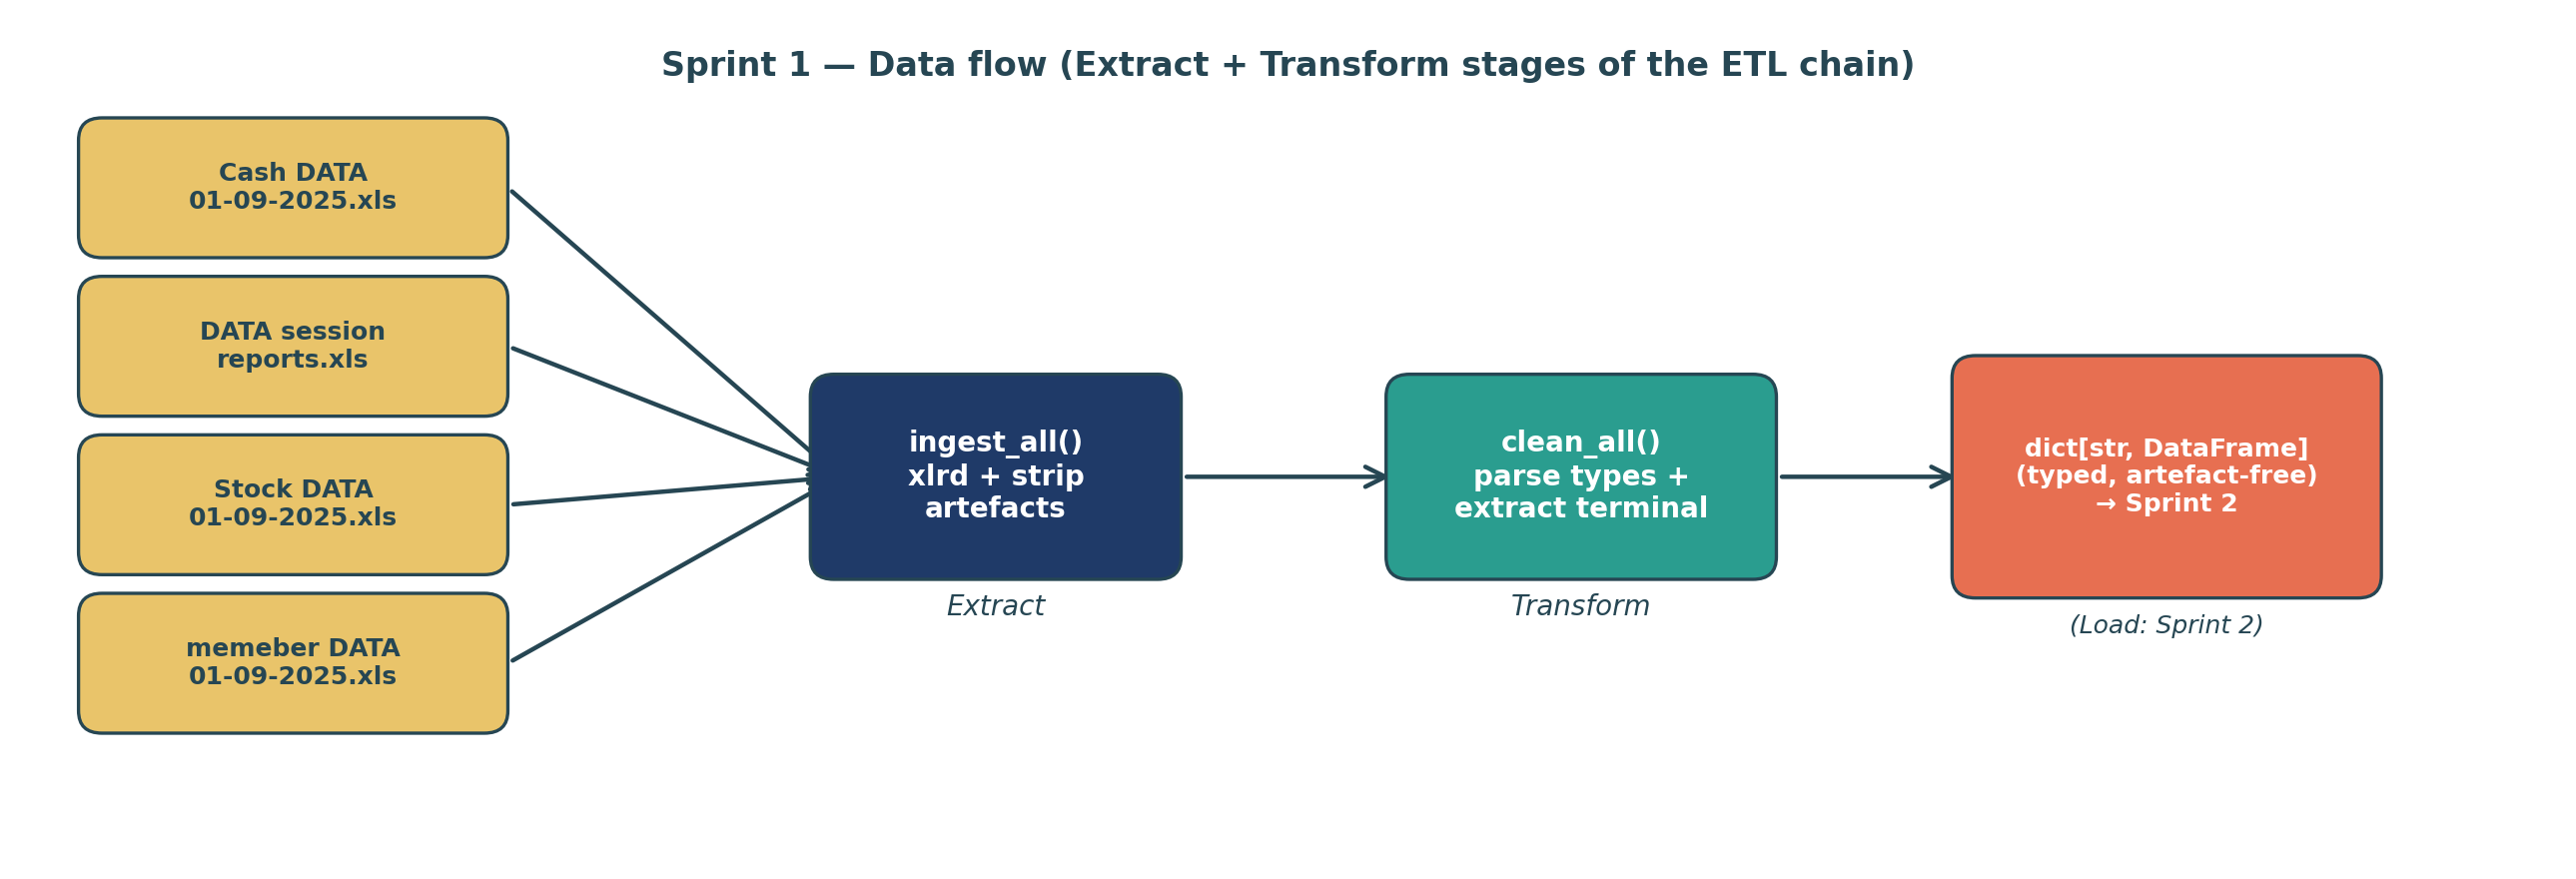
\includegraphics[width=0.85\textwidth]{images/sprint1_flow.png}
  \caption{Data flow of Sprint~1: ingestion and cleaning.}
  \label{fig:sprint1_flow}
\end{figure}

The choice of \texttt{xlrd} over \texttt{pandas.read\_excel} is the most
visible peculiarity of the chain and is justified in detail in the next
section. The choice of a string-only output from the ingestor is also
deliberate: keeping the conversions in a dedicated cleaning module makes
each parser unit-testable in isolation and prevents type errors from
silently propagating through the rest of the chain.

% ----------------------------------------------------------
\section{Implementation of the Ingestion Stage}

\subsection{Overview}

The ingestion stage is implemented in \texttt{gamefydb/ingestor.py}. Its
responsibility is to produce one clean, artefact-free DataFrame per source file,
using only the columns that carry genuine data. Three design decisions shaped the
implementation:

\begin{itemize}
  \item \textbf{xlrd instead of pandas.} The members file (\texttt{memeber DATA
        01-09-2025.xls}) triggers a \texttt{charmap} codec error when opened with
        \texttt{pandas.read\_excel}. Reading each file at the \texttt{xlrd}
        workbook level and reconstructing a DataFrame from \texttt{ws.row\_values()}
        bypasses the codec path entirely and works for all four files uniformly.

  \item \textbf{Empirical column mapping.} Excel's merged cells cause the visible
        column headers to sit at different indices than the actual data cells when
        the file is read as a flat matrix. For example, the \texttt{comment} column
        in the cash file has its header at index~50 but its data at index~51. The
        \texttt{COLUMN\_MAPS} dictionary stores the verified data positions for every
        column of every file.

  \item \textbf{Artefact stripping.} All four files contain periodic page-break
        sequences — a \textit{Page X/Y} marker row, two blank rows, and a full
        header repetition — inserted roughly every 40 data rows by the export
        software. These must be removed before any type conversion is attempted.
\end{itemize}

Figure~\ref{fig:raw_xls} shows what one of these files looks like when
opened directly in Excel, with the page-break artefacts highlighted in
red. This is the input the pipeline starts from.

\begin{figure}[H]
  \centering
  \todoFigure[0.85\textwidth]{Screenshot of \texttt{14-06-2025 cash.xls}
  opened in Excel, with at least one page-break sequence
  (\textit{Page~X/Y} row + two blank rows + repeated header) highlighted
  in red. Crop to about 25--30 rows so the artefact is visible.}
  \caption{Raw \texttt{.xls} export, with page-break artefacts visible.}
  \label{fig:raw_xls}
\end{figure}

\subsection{Reading the Raw File}

Listing~\ref{lst:read_raw} shows the \texttt{\_read\_raw()} helper that converts
an \texttt{.xls} file into a header-free pandas DataFrame.

\begin{lstlisting}[
  language=Python,
  caption={Reading an \texttt{.xls} file with \texttt{xlrd}.},
  label={lst:read_raw},
  basicstyle=\ttfamily\small,
  keywordstyle=\bfseries,
  frame=single,
  breaklines=true
]
def _read_raw(path: str) -> pd.DataFrame:
    wb = xlrd.open_workbook(path)
    ws = wb.sheet_by_index(0)
    data = [ws.row_values(i) for i in range(ws.nrows)]
    wb.release_resources()
    return pd.DataFrame(data)
\end{lstlisting}

Every row of the worksheet — including title rows, blank rows, and header rows —
is loaded into the DataFrame with no interpretation. Index values correspond
directly to xlrd column positions, making the mapping in \texttt{COLUMN\_MAPS}
precise and unambiguous.

\subsection{Column Maps}

The \texttt{COLUMN\_MAPS} dictionary (Listing~\ref{lst:colmaps}) centralises all
column-position knowledge for the four source files. Each entry maps a
0-indexed \texttt{xlrd} column position to the canonical output column name used
throughout the rest of the pipeline.

\begin{lstlisting}[
  language=Python,
  caption={\texttt{COLUMN\_MAPS} — empirically verified column positions.},
  label={lst:colmaps},
  basicstyle=\ttfamily\small,
  keywordstyle=\bfseries,
  frame=single,
  breaklines=true
]
COLUMN_MAPS = {
    'cash': {
        0: 'cashier',   4: 'date',      9: 'income_expense',
       11: 'payment_method',           21: 'transaction_type',
       40: 'amount',                   51: 'comment',
    },
    'sessions': {
        0: 'cashier',   4: 'terminal',  9: 'session_type',
       12: 'free_time', 14: 'paused',  20: 'duration',
       22: 'order_transfer',           28: 'usage',
       30: 'discount',                 32: 'total_amount',
    },
    'stock': {
        0: 'cashier',   4: 'date',      8: 'item_name',
       13: 'category', 20: 'in_out',   25: 'quantity',
       28: 'unit_price',               29: 'total_amount',
       32: 'comment',
    },
    'members': {
        2: 'member_id', 6: 'username',  8: 'firstname',
       13: 'lastname',                 14: 'duration',
       22: 'usage',                    27: 'orders_transfer',
       30: 'total_amount',
    },
}
\end{lstlisting}

The positions were determined by calling \texttt{ws.row\_values()} on a known
data row in each file and inspecting the output manually. They must not be
adjusted without re-verifying against the raw source file, because any future
change to the export format could shift all subsequent columns.

\subsection{Artefact Stripping}

The \texttt{\_strip\_artifacts()} function (Listing~\ref{lst:strip}) removes all
non-data rows from a raw DataFrame in a fixed sequence of steps:

\begin{enumerate}
  \item \textbf{Skip the file header block} — the first five rows of every file
        are a title row, a report-date row, and three blank/header rows that are
        always present and never contain data.
  \item \textbf{Remove page-marker rows} — any row containing a cell that matches
        the regular expression \texttt{Page~\textbackslash d+/\textbackslash d+}
        is dropped. This pattern appears in all four files.
  \item \textbf{Remove repeated header rows} — the export software repeats the
        column headers at the top of each new page. These rows have the text
        \texttt{"Cashier"} in the first mapped column and are dropped by equality
        check.
  \item \textbf{Select and rename mapped columns} — only the columns listed in
        \texttt{COLUMN\_MAPS} are retained; they are renamed to their canonical names.
  \item \textbf{Drop remaining blank or footer rows} — rows where the designated
        key column (e.g., \texttt{date} for cash and stock, \texttt{terminal} for
        sessions, \texttt{member\_id} for members) is empty or NaN are discarded.
\end{enumerate}

\begin{lstlisting}[
  language=Python,
  caption={Artefact stripping in \texttt{\_strip\_artifacts()}.},
  label={lst:strip},
  basicstyle=\ttfamily\small,
  keywordstyle=\bfseries,
  frame=single,
  breaklines=true
]
PAGE_PATTERN = re.compile(r'Page \d+/\d+')

def _strip_artifacts(df, col_map, key_col):
    # 1. skip the 5-row file header block
    df = df.iloc[5:].reset_index(drop=True)

    # 2. drop page-marker rows
    has_page = df.apply(
        lambda row: any(PAGE_PATTERN.search(str(v)) for v in row),
        axis=1,
    )
    df = df[~has_page].reset_index(drop=True)

    # 3. drop repeated header rows
    first_idx = min(col_map.keys())
    df = df[
        df.iloc[:, first_idx].astype(str).str.strip() != 'Cashier'
    ].reset_index(drop=True)

    # 4. select and rename mapped columns
    df = df[list(col_map.keys())].rename(columns=col_map)

    # 5. drop footer / blank rows via key column
    key = df[key_col]
    mask = key.notna() & (key.astype(str).str.strip() != '')
    return df[mask].reset_index(drop=True)
\end{lstlisting}

A special case arises for the members file: the last row of the report is a
footer row with the text \texttt{"Report Result\,:"} in a label cell. This row
passes the key-column check because \texttt{member\_id} is present as a numeric
total. It is filtered out later in the cleaning stage by coercing \texttt{member\_id}
to numeric with \texttt{errors='coerce'} and dropping the resulting NaN rows.

\subsection{The \texttt{ingest\_all()} Entry Point}

The public interface of the ingestion stage is \texttt{ingest\_all()}, which
applies \texttt{\_read\_raw()} and \texttt{\_strip\_artifacts()} to each of the
four files and returns a dictionary of clean raw DataFrames:

\begin{lstlisting}[
  language=Python,
  caption={Public entry point of the ingestion stage.},
  label={lst:ingestall},
  basicstyle=\ttfamily\small,
  keywordstyle=\bfseries,
  frame=single,
  breaklines=true
]
def ingest_all(input_dir: str) -> dict:
    base = input_dir.rstrip('/').rstrip('\\')
    result = {}
    for name, filename in FILE_MAP.items():
        path = f"{base}/{filename}"
        df_raw = _read_raw(path)
        result[name] = _strip_artifacts(
            df_raw, COLUMN_MAPS[name], KEY_COLS[name]
        )
    return result
\end{lstlisting}

At this point all values remain as strings (or floats for cells that xlrd
interpreted as numbers). Type normalisation is the responsibility of the cleaning
stage, described in Section~\ref{sec:cleaning}.

% ----------------------------------------------------------
\section{Implementation of the Cleaning Stage}
\label{sec:cleaning}

\subsection{Overview}

The cleaning stage is implemented in \texttt{gamefydb/cleaner.py}. It receives
the dictionary of raw DataFrames produced by \texttt{ingest\_all()} and returns
a dictionary of fully typed DataFrames in which every column has the correct
Python / pandas type. Four categories of conversion are needed across the four
files:

\begin{itemize}
  \item \textbf{Monetary amounts} — TND values encoded with a narrow no-break
        space (\texttt{\textbackslash u202f}) as the thousands separator and a
        comma as the decimal separator (e.g., \texttt{1\,745,44 TND}).
  \item \textbf{Datetimes} — strings in \texttt{DD.MM.YYYY HH:MM:SS} format
        present in the cash and stock files.
  \item \textbf{Durations} — human-readable strings such as \texttt{1\,h\,29\,min}
        or \texttt{30\,min} that must be converted to integer total minutes.
  \item \textbf{Terminal names} — in the cash and stock files the terminal is
        stored as a parenthesised comment like \texttt{(GAMEFY01)} or
        \texttt{(PS5\,(1))}. The name must be extracted from the outermost parens.
\end{itemize}

\subsection{Parsing Helpers}

Four pure functions implement the individual conversions.

\paragraph{parse\_amount()} strips the thousands separator and the \texttt{TND}
suffix, then replaces the comma decimal separator with a period before converting
to \texttt{float}:

\begin{lstlisting}[
  language=Python,
  caption={\texttt{parse\_amount()} — TND amount parser.},
  label={lst:parse_amount},
  basicstyle=\ttfamily\small,
  keywordstyle=\bfseries,
  frame=single,
  breaklines=true
]
def parse_amount(value: str) -> float:
    s = (str(value)
         .replace('\u202f', '')   # narrow no-break space (thousands sep)
         .replace(' TND', '')
         .replace(',', '.'))
    return float(s)
\end{lstlisting}

\paragraph{parse\_datetime()} delegates to \texttt{datetime.strptime} with the
fixed format string \texttt{\%d.\%m.\%Y \%H:\%M:\%S}:

\begin{lstlisting}[
  language=Python,
  caption={\texttt{parse\_datetime()} — datetime parser.},
  label={lst:parse_datetime},
  basicstyle=\ttfamily\small,
  keywordstyle=\bfseries,
  frame=single,
  breaklines=true
]
def parse_datetime(value: str) -> datetime:
    return datetime.strptime(str(value).strip(), '%d.%m.%Y %H:%M:%S')
\end{lstlisting}

\paragraph{parse\_duration()} uses a regular expression to capture optional hours
and mandatory minutes, then computes the total in minutes:

\begin{lstlisting}[
  language=Python,
  caption={\texttt{parse\_duration()} — duration parser.},
  label={lst:parse_duration},
  basicstyle=\ttfamily\small,
  keywordstyle=\bfseries,
  frame=single,
  breaklines=true
]
_DURATION_RE = re.compile(r'(?:(\d+)\s*h\s*)?(\d+)\s*min')

def parse_duration(value: str) -> int:
    m = _DURATION_RE.search(str(value))
    if not m:
        raise ValueError(f"Cannot parse duration: {value!r}")
    hours = int(m.group(1)) if m.group(1) else 0
    return hours * 60 + int(m.group(2))
\end{lstlisting}

\paragraph{extract\_terminal()} matches only the outermost pair of parentheses,
so that terminal names such as \texttt{PS5\,(1)} — which contain an inner pair —
are captured correctly:

\begin{lstlisting}[
  language=Python,
  caption={\texttt{extract\_terminal()} — terminal name extractor.},
  label={lst:extract_terminal},
  basicstyle=\ttfamily\small,
  keywordstyle=\bfseries,
  frame=single,
  breaklines=true
]
_TERMINAL_RE = re.compile(r'^\((.+)\)$')

def extract_terminal(value) -> str | None:
    if value is None or (isinstance(value, float) and pd.isna(value)):
        return None
    m = _TERMINAL_RE.match(str(value).strip())
    return m.group(1) if m else None
\end{lstlisting}

\subsection{Per-File Cleaning Functions}

Each of the four DataFrames requires a slightly different set of transformations.
The per-file cleaning functions apply the helpers and handle any file-specific
edge cases.

\paragraph{\_clean\_cash()} strips cashier names, parses dates and amounts, and
extracts the terminal name from the \texttt{comment} column:

\begin{lstlisting}[
  language=Python,
  caption={Cleaning the cash DataFrame.},
  label={lst:clean_cash},
  basicstyle=\ttfamily\small,
  keywordstyle=\bfseries,
  frame=single,
  breaklines=true
]
def _clean_cash(df):
    out = df.copy()
    out['cashier']    = out['cashier'].str.strip()
    out['date']       = pd.to_datetime(out['date'],
                            format='%d.%m.%Y %H:%M:%S')
    out['amount_tnd'] = out['amount'].apply(parse_amount)
    out['terminal']   = out['comment'].apply(extract_terminal)
    return out.drop(columns=['amount'])
\end{lstlisting}

\paragraph{\_clean\_sessions()} is the most complex cleaner because the sessions
file has no \texttt{comment} column — terminal names arrive directly as plain
strings, not wrapped in parentheses. It also parses four TND columns, a duration,
and two boolean-like marker columns (\texttt{free\_time} and \texttt{paused}):

\begin{lstlisting}[
  language=Python,
  caption={Cleaning the sessions DataFrame.},
  label={lst:clean_sessions},
  basicstyle=\ttfamily\small,
  keywordstyle=\bfseries,
  frame=single,
  breaklines=true
]
def _clean_sessions(df):
    out = df.copy()
    out['cashier']  = out['cashier'].str.strip()
    out['terminal'] = out['terminal'].str.strip()
    out['duration_minutes'] = out['duration'].apply(parse_duration)
    out['is_free_time'] = out['free_time'].apply(_has_marker)
    out['paused_duration_minutes'] = out['paused'].apply(
        lambda v: parse_duration(v) if _has_marker(v) else None
    )
    for src, dst in [
        ('order_transfer', 'order_transfer_tnd'),
        ('usage',          'usage_tnd'),
        ('discount',       'discount_tnd'),
        ('total_amount',   'total_amount_tnd'),
    ]:
        out[dst] = out[src].apply(parse_amount)
    return out.drop(columns=[
        'duration', 'free_time', 'paused',
        'order_transfer', 'usage', 'discount', 'total_amount',
    ])
\end{lstlisting}

\paragraph{\_clean\_stock()} follows the same pattern as cash: dates, amounts, and
terminal extraction from \texttt{comment}. Quantity is additionally cast to integer:

\begin{lstlisting}[
  language=Python,
  caption={Cleaning the stock DataFrame.},
  label={lst:clean_stock},
  basicstyle=\ttfamily\small,
  keywordstyle=\bfseries,
  frame=single,
  breaklines=true
]
def _clean_stock(df):
    out = df.copy()
    out['cashier']         = out['cashier'].str.strip()
    out['date']            = pd.to_datetime(out['date'],
                                 format='%d.%m.%Y %H:%M:%S')
    out['quantity']        = pd.to_numeric(out['quantity']).astype(int)
    out['unit_price_tnd']  = out['unit_price'].apply(parse_amount)
    out['total_amount_tnd']= out['total_amount'].apply(parse_amount)
    out['terminal']        = out['comment'].apply(extract_terminal)
    return out.drop(columns=['unit_price', 'total_amount'])
\end{lstlisting}

\paragraph{\_clean\_members()} handles the footer-row edge case: coercing
\texttt{member\_id} to numeric with \texttt{errors='coerce'} converts the
\texttt{"Report Result\,:"} footer cell to NaN, and \texttt{dropna} then removes
it automatically:

\begin{lstlisting}[
  language=Python,
  caption={Cleaning the members DataFrame.},
  basicstyle=\ttfamily\small,
  keywordstyle=\bfseries,
  frame=single,
  breaklines=true
]
def _clean_members(df):
    out = df.copy()
    out['member_id'] = pd.to_numeric(out['member_id'], errors='coerce')
    out = out.dropna(subset=['member_id']).copy()
    out['member_id'] = out['member_id'].astype(int)
    out['duration_minutes']     = out['duration'].apply(parse_duration)
    out['usage_tnd']            = out['usage'].apply(parse_amount)
    out['orders_transfer_tnd']  = out['orders_transfer'].apply(parse_amount)
    out['total_amount_tnd']     = out['total_amount'].apply(parse_amount)
    return out.drop(columns=[
        'duration', 'usage', 'orders_transfer', 'total_amount'
    ])
\end{lstlisting}

\subsection{The \texttt{clean\_all()} Entry Point}

The public interface of the cleaning stage is \texttt{clean\_all()}, which
dispatches each raw DataFrame to its dedicated cleaning function and returns a
dictionary with the same four keys:

\begin{lstlisting}[
  language=Python,
  caption={\texttt{clean\_all()} — public entry point of the cleaning stage.},
  label={lst:cleanall},
  basicstyle=\ttfamily\small,
  keywordstyle=\bfseries,
  frame=single,
  breaklines=true
]
def clean_all(raw: dict) -> dict:
    return {
        'cash':     _clean_cash(raw['cash']),
        'sessions': _clean_sessions(raw['sessions']),
        'stock':    _clean_stock(raw['stock']),
        'members':  _clean_members(raw['members']),
    }
\end{lstlisting}

At the exit of \texttt{clean\_all()} every column has its correct native type:
\texttt{datetime64} for all date fields, \texttt{float64} for monetary amounts,
\texttt{int64} for durations and member identifiers, and \texttt{object} (string)
for names and categorical labels. Figure~\ref{fig:cleaned_df} shows the resulting
DataFrame for the cash file as inspected in a Jupyter session.

\begin{figure}[H]
  \centering
  \todoFigure[0.85\textwidth]{Screenshot from a Jupyter notebook of the
  cleaned cash DataFrame: run \texttt{clean\_all(ingest\_all("excel"))["cash"].head(10)}
  and follow it with \texttt{.dtypes} so both the values and the column
  types are visible in the same crop.}
  \caption{Cleaned cash DataFrame after \texttt{clean\_all()}.}
  \label{fig:cleaned_df}
\end{figure}

% ----------------------------------------------------------
\section{Sprint 1 Review}

\subsection{Deliverables}

The following deliverables were produced and validated at the Sprint~1 review:

\begin{itemize}
  \item \textbf{\texttt{gamefydb/ingestor.py}} — fully functional ingestion stage
        that reads all four \texttt{.xls} files via \texttt{xlrd}, strips all
        page-break artefacts, and returns artefact-free string DataFrames.
  \item \textbf{\texttt{gamefydb/cleaner.py}} — fully functional cleaning stage
        with four parsing helpers and four per-file cleaning functions that produce
        typed DataFrames.
  \item \textbf{Automated tests} — \texttt{pytest} test suite covering each helper
        function and each per-file cleaner with sample inputs.
\end{itemize}

\subsection{Validation}

Validation was performed by running the pipeline end-to-end from the command line
and inspecting the intermediate DataFrames at the exit of \texttt{clean\_all()}.
The following checks were applied:

\begin{itemize}[noitemsep]
  \item Row counts match the expected number of transactions, sessions, stock
        movements, and members after artefact stripping.
  \item No \texttt{NaN} values appear in mandatory columns (amounts, dates,
        cashier names, terminal names for sessions).
  \item The \texttt{dtypes} attribute of each DataFrame confirms correct types
        for every column.
  \item Terminal names extracted from cash and stock comments match the canonical
        names used directly in the sessions file (e.g., \texttt{GAMEFY01},
        \texttt{PS5\,(1)}, \texttt{GAMEFY-VIP}).
\end{itemize}

% ----------------------------------------------------------
\section{Conclusion}

Sprint~1 delivered a robust, fully tested ingestion and cleaning layer that
transforms the four raw \texttt{.xls} files into typed, artefact-free DataFrames.
All encoding issues, page-break artefacts, non-standard separators, and footer
rows have been handled at the source. The output of this sprint provides a solid
foundation for the dimensional modelling work that follows in Sprint~2, which is
described in Chapter~4.
